\documentclass[11pt,a4paper]{article}
% ============================================================
% Shared preamble for Claude Experiments reports (Ukrainian, LuaLaTeX)
% Compile with: lualatex report_*_uk.tex
% Include this AFTER \documentclass in each report:
%   \documentclass[11pt,a4paper]{article}
%   \input{../preamble_uk}
% ============================================================
% Cyrillic via LuaLaTeX + fontspec (pdflatex has no T2A here).
\usepackage{fontspec}
\setmainfont{DejaVu Serif}
\setsansfont{DejaVu Sans}
\setmonofont{DejaVu Sans Mono}
\usepackage[a4paper,top=2.5cm,bottom=2.5cm,left=2.5cm,right=2.5cm]{geometry}
\usepackage{amsmath,amssymb}
\usepackage{graphicx}
\usepackage{subcaption}
\usepackage{booktabs}
\usepackage{xcolor}
\usepackage[colorlinks=true,allcolors=blue]{hyperref}
\usepackage{microtype}
\usepackage{float}
\usepackage{array}
\microtypesetup{expansion=false}

% Color scheme
\definecolor{colMicro}{HTML}{222222}
\definecolor{colExact}{HTML}{2878b5}
\definecolor{colPlacement}{HTML}{e07a1f}
\definecolor{colBoundary}{HTML}{429c74}
\definecolor{colCurrent}{HTML}{c23b55}
\definecolor{colMM}{HTML}{c23b55}

\providecommand{\SIG}{\textcolor{green!50!black}{\textbf{*}}}
\providecommand{\NS}{\textcolor{gray}{n.s.}}
\providecommand{\DRMS}{\Delta\mathrm{RMST}}
\providecommand{\ci}[2]{$[{#1},\;{#2}]$}

\usepackage{longtable}
\setlength{\emergencystretch}{2em}

\title{\textbf{Коли MicroMacro відрізняється від Full Micro:}\\
синтез результатів і наслідки для калібрування}
\author{Two-Layer CTMC Research Synthesis}
\date{4 серпня 2026}

\begin{document}
\maketitle

\begin{abstract}
Цей звіт комплексно синтезує аналітичні benchmarks, завершені та
development-експерименти з порівняння
повного Gillespie CTMC (Full Micro) і дворівневого симулятора MicroMacro.
Основна мета --- не знайти одну середню похибку, а встановити, у яких режимах
два методи узгоджуються, де виникає систематичне зміщення і які агрегатні
дескриптори можуть керувати майбутнім калібруванням. Сукупні результати
показують, що найкраще підтверджений механізм premature discrepancy ---
накопичення aggregate hazard до досягнення інфекцією export-relevant boundary
nodes, але його outcome-level внесок залежить від scheduler і regime.
Величина і навіть знак похибки визначаються співвідношенням швидкості export
до внутрішнього mixing, щільністю спільнот, шириною interface, recovery та
топологією. Жодна перевірена always-on correction не є безпечною в усіх
режимах. Практичний наслідок --- калібрування має бути regime-aware,
sign-aware, censoring-aware, мати identity gate для добре перемішаних мереж
і проходити minimax validation на різних topology families.
\end{abstract}

\tableofcontents
\clearpage

\section{Мета та рамка аналізу}

Full Micro моделює всі внутрішні та міжспільнотні transmission events на
explicit contact network. MicroMacro залишає точний micro-level Gillespie
всередині спільнот, але замінює explicit inter-community edges агрегованим
hazard
\[
 \lambda_{ij}(t)=\beta_{out}T W_{ij}
 \frac{I_i(t)}{N_i}\frac{S_j(t)}{N_j},
\]
після чого розміщує import рівномірно серед susceptible nodes destination
community. Питання дослідження формулюється так:

\begin{quote}
За яких network/epidemic regimes ця заміна відтворює arrival-time process
Full Micro, а за яких --- створює practically significant bias, який можна
передбачити й зменшити за доступними macro-level descriptors?
\end{quote}

Одиницею статистичного спостереження в усіх коректно побудованих порівняннях
є replication. Основні метрики:
\begin{itemize}
 \item $\Delta\mathrm{RMST}=\mathrm{RMST}_{MM}-\mathrm{RMST}_{Micro}$ ---
 censoring-aware timing shift; від'ємне значення означає premature arrival;
 \item $\Delta\mathrm{RMST}/T_{end}$ --- порівнювана між різними horizons метрика;
 \item relative $W_1$ --- completed-only distributional discrepancy;
 \item $\Delta p=p_{MM}-p_{Micro}$ --- різниця completion probabilities;
 \item layer-wise paired error $T_i^{MM}-T_i^{Micro}$ --- накопичення похибки.
\end{itemize}

Completed-only $W_1$ не використовується окремо від completion. За різних
horizons сирі RMST або arrival means не порівнюються між сценаріями.

\section{Позначення}

\small
\setlength{\tabcolsep}{4pt}
\begin{longtable}{p{3.0cm}p{7.0cm}p{4.3cm}}
\toprule
Позначення & Визначення & Інтерпретація у звіті\\
\midrule
\endhead
Micro / Full Micro & Повний Gillespie CTMC на explicit contact network & Reference або ground truth.\\
MicroMacro / MM & Дворівневий simulator з exact local dynamics та aggregate inter-community hazard & Апроксимація, яку порівнюємо з Micro.\\
$L$ & Кількість communities у chain & Terminal community має index $L-1$.\\
$N_i$, $n$ & Розмір community $i$; $n$ --- спільний розмір в однорідних scenarios & Наприклад, $n=100$.\\
$d$ & Середній internal node degree & Більше $d$ зазвичай означає швидше local mixing.\\
$k$ & Кількість explicit inter-community edges між сусідніми communities & Interface width; його effect не обов'язково монотонний.\\
$W_{ij}$ & Aggregate inter-community weight від $i$ до $j$ & У chain benchmarks зазвичай $W_{ij}=k$.\\
$\beta_{in}$ & Transmission rate на internal edges & Визначає швидкість поширення всередині community.\\
$\beta_{out}$ & Transmission rate на explicit inter-community edges & Визначає microscopic export clock.\\
$\beta_{macro}$ & Rate coefficient aggregate macro hazard & Часто встановлено $\beta_{macro}=\beta_{out}$.\\
$r=\beta_{out}/\beta_{in}$ & Export-to-internal-transmission ratio & Велике $r$: export конкурує з mixing; мале $r$: export повільний.\\
$\gamma$ & Recovery rate & $\gamma=0$ відповідає SI; $\gamma>0$ --- SIR.\\
$R_0$ & Epidemic reproduction proxy, у CE-04 заданий через rates & Менше $R_0$ збільшує extinction і censoring.\\
$\tau_{micro}$ & Synchronization interval MicroMacro & Baseline переважно використовує $\tau_{micro}=1$.\\
$T$, $T_{end}$ & $T$ --- macro scaling factor; $T_{end}$ --- simulation horizon & Arrival після $T_{end}$ вважається censored.\\
$I_i(t),S_i(t)$ & Кількість infected і susceptible у community $i$ & $\bar i_i=I_i/N_i$, $\bar s_i=S_i/N_i$.\\
$\lambda_{ij}(t)$ & Aggregate macro import hazard & $\beta_{out}T W_{ij}\bar i_i(t)\bar s_j(t)$.\\
$a^*_{ij}(t)$ & Exact active-edge inter-community hazard & Сума propensities лише активних infected--susceptible bridge edges.\\
$B_I(t)$ & Кількість infected boundary/bridge nodes & При $B_I=0$ exact export hazard може бути zero.\\
$T_i$ & First infection arrival time у community $i$ & Layer-wise propagation timing.\\
$T_{last}=T_{L-1}$ & Arrival time до останньої community & Основний terminal outcome.\\
$\Delta T_i=T_{i+1}-T_i$ & Local delay між сусідніми communities & Не плутати з cumulative paired error.\\
$T_i^{MM}-T_i^{Micro}$ & Paired cumulative arrival error від simulation start & Negative означає раніше прибуття MM.\\
Completion & Частка runs, де $T_{last}<T_{end}$ & Завжди подається разом із completed-only metrics.\\
$W_1$ & Wasserstein-1 distance між empirical arrival distributions & Вимірюється в одиницях часу.\\
relative $W_1$ & $W_1/\mathbb E[T^{Micro}]$ & Безрозмірна distributional discrepancy.\\
RMST & $\mathbb E[\min(T_{last},T_{end})]$ & Censoring-aware terminal timing.\\
$\Delta\mathrm{RMST}$ & $\mathrm{RMST}_{MM}-\mathrm{RMST}_{Micro}$ & Negative: premature MM; positive: late MM.\\
$\Delta\mathrm{RMST}/T_{end}$ & Horizon-normalized RMST shift & Для обережного cross-scenario порівняння.\\
$\Delta p$ & $p_{MM}-p_{Micro}$ & Completion-probability mismatch.\\
$\mu_2$ & Fiedler value normalized graph Laplacian & Parameters-only proxy internal connectivity/mixing.\\
$\lambda_1$, $\ell$ & Spectral radius і average shortest-path length & Використовуються у spectral lag/latent corrections.\\
$c^*$ & Оптимальний scalar multiplier для $\beta_{macro}$ у CE-07 & Pilot estimate; не універсальна константа.\\
Gap closure & Частка baseline error, прибрана correction & $1$: gap закрито; $0$: без зміни; $<0$: regression.\\
CI / IQR & Confidence interval / interquartile range & CI описує uncertainty; IQR --- variability між runs.\\
\bottomrule
\end{longtable}
\normalsize

\section{Карта доказів}

\begin{longtable}{p{2.1cm}p{4.0cm}p{2.1cm}p{6.0cm}}
\toprule
ID & Питання & Статус & Роль у синтезі\\
\midrule
\endhead
B00 & Clique--bridge--leaf & theory + numerical & Мінімальна boundary-модель і Jensen timing mechanism.\\
B01 & Chain of cliques & завершено & Well-mixed baseline і накопичення timing error.\\
B02 & Sparse connected chain & завершено & Основний production stress case premature leakage.\\
Exp-01 (CE-01 report) & Hazard--placement ablation & final, 100 & Один dataset: causal decomposition hazard і placement mechanisms.\\
Exp-02 & State-replay hazard audit & final, 100 & Formula mismatch на спільних Full Micro states.\\
CE-03 / CE-11 & Export-ratio sweep & завершено & Sign change як функція $r=\beta_{out}/\beta_{in}$.\\
CE-04 & SIR validation & завершено & Recovery, censoring та false completion.\\
CE-06 & Regime map & full, 36 cells & Спільний вплив $r,d,k$.\\
CE-07 & Calibration floor & pilot & Частка removable scalar-rate error; оцінка оптимістична.\\
CE-08 & Dense negative control & final, 200 & Перевірка identity/well-mixed regime.\\
CE-09 & Boundary diagnostic & full & Placement proxy; modes не network-paired.\\
CE-10 & Spectral correction & full, 12 cells & Де spectral damping допомагає або шкодить.\\
CE-12 & Statistical power & planned & Даних ще немає; 100 runs можуть бути under-powered.\\
Exp-05 & Spectral lag/latent state & validation & Development evidence; literal corrections не пройшли.\\
ER-01 & Multi-topology validation & smoke; pilot active & Generalization gate; pilot не інтерпретується до завершення.\\
\bottomrule
\end{longtable}

\section{Аналітичний boundary benchmark}

Clique--bridge--leaf construction є найпростішою моделлю втрати boundary
information. Source community є clique $K_n$, але export до leaf можливий лише
через bridge set $B$ розміру $k$. Exact microscopic hazard дорівнює
\[
 a^{Micro}_{01}(t)=\beta_{out}B_I(t),
\]
де $B_I(t)$ --- кількість інфікованих bridge nodes. До першої bridge activation
$T_B$ exact hazard є нульовим незалежно від загального $I(t)$. Для одного bridge
в SI процесі
\[
 T_A=T_B+Z,\qquad Z\sim\mathrm{Exp}(\beta_{out}),
\]
що явно розділяє boundary-finding delay і post-boundary export clock.

Macro layer замінює невідомий $B_I(t)$ на $kI(t)/n$. За exchangeability ця
величина може бути коректним conditional mean exact hazard, але це не гарантує
правильний event-time distribution. Через convexity $\exp(-x)$ conditional
Jensen inequality дає більшу exact survival probability, тобто mean-field
clock може давати premature export навіть за правильного instantaneous mean.
Це теоретична основа всієї статті: boundary information loss впливає на
накопичений hazard, а не лише на середню rate.

Numerical clique--bridge--leaf benchmark з $n=100$ і $k=2$ показав лише
помірну практичну різницю. Bridge nodes у clique активуються швидко, тоді як
довгий exponential post-bridge waiting time домінує у total-export variance і
маскує частину structural bias. Отже, наявність механізму не означає великої
outcome discrepancy в кожному regime.

\begin{figure}[H]
 \centering
 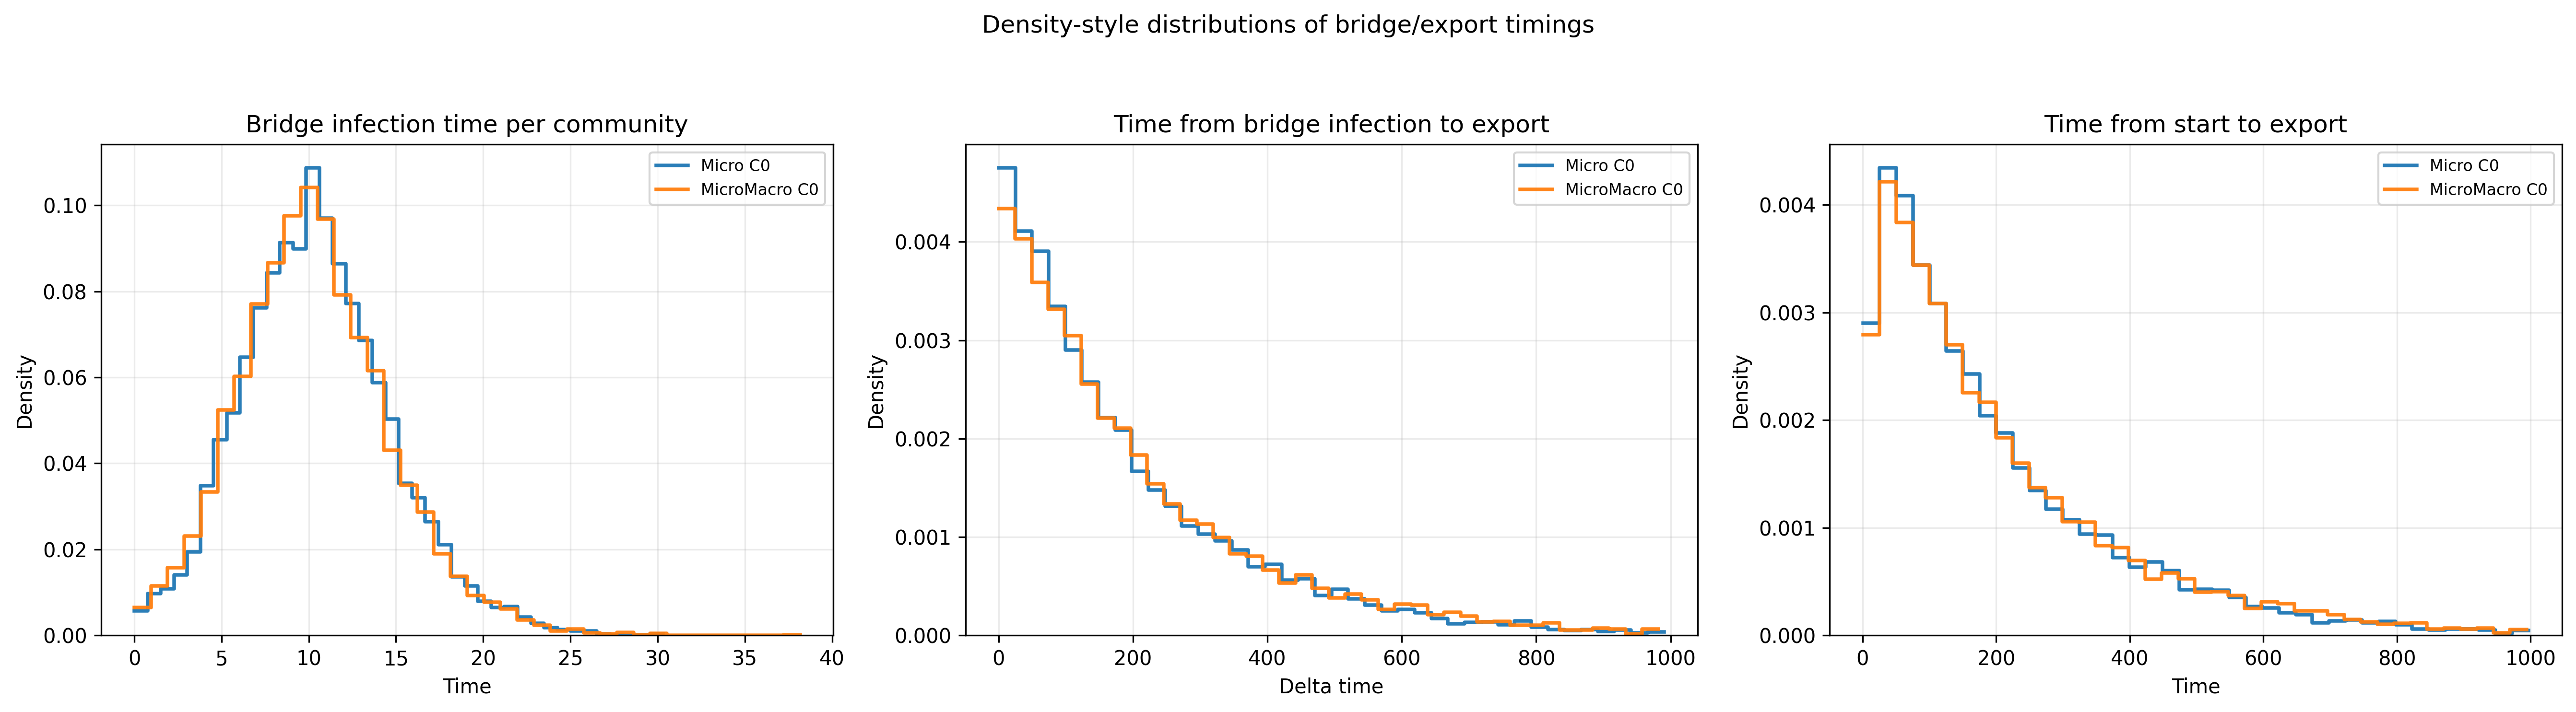
\includegraphics[width=.9\linewidth]{../../paper/Images/research_synthesis/clique_bridge_leaf_timing.png}
 \caption{Clique--bridge--leaf timing decomposition з основної статті:
 bridge activation, post-bridge export delay і total export time. Це
 minimal boundary benchmark, а не chain-level stress test.}
\end{figure}

\section{Сумірність усіх джерел доказів}

Експерименти відповідають на різні питання і не є повтореннями однієї grid.
Таблиця нижче визначає межі коректного спільного аналізу. Exp-01 і CE-01 є
одним ablation dataset та не рахуються двома незалежними підтвердженнями.

\begin{longtable}{p{2.25cm}p{4.25cm}p{1.45cm}p{2.35cm}p{4.6cm}}
\toprule
Evidence & Основний дизайн & Runs & Статус & Що ідентифікує\\
\midrule
\endhead
B00 & clique--bridge--leaf, $n=100,k=2$ & article benchmark & final & Boundary mechanism у мінімальній topology.\\
B01 & clique chain; $L=10,n=100$; $\beta=.001$ & 100/cell & final & Production full-system error у fast-mixing communities.\\
B02 & connected ER chain; $d,k$ sweeps; $\beta=.003$ & 100/cell & final & Production stress behavior за sparse mixing.\\
Exp-01/CE-01 & exact/aggregate hazard та exact/boundary/uniform placement & 100 paired & final & Causal contrasts у event-driven architecture.\\
Exp-02 & exact та aggregate hazards на тих самих Full Micro states & 100 replay & final & Formula-level rate mismatch без trajectory confounding.\\
CE-03/11 & $r\in\{.1,.3,1,2,5\}$; різні horizons, normalized re-analysis & 100/cell & final & Sign change за export-to-mixing ratio.\\
CE-04 & $\gamma\in\{0,.0005,.001,.003\}$ & 100/cell & final & Recovery і completion failure.\\
CE-06 & $r\times d\times k$: 36 cells & 60/cell & final & Regime map у random-connected SI family.\\
CE-07 & scalar $\beta_{macro}$ calibration, 9 cells & 40/cell & pilot & In-sample calibration floor; не generalization.\\
CE-08 & chain із трьох $K_{100}$, $k=2$ & 200 & final & Dense negative control.\\
CE-09 & boundary placement diagnostics, 6 regimes & 40/cell & final, unpaired modes & Static boundary proxy; не causal effect.\\
CE-10 & spectral/availability corrections, 12 cells & 60/cell & final & Regime-dependent correction benefit/regression.\\
Exp-05 & lag/latent corrections, sparse baseline & 20 validation; 100 snapshot & development & Literal formula rejection на baseline; sweeps incomplete.\\
ER-01 & topology transfer: chain/complete $\times$ three micro families & 8/cell smoke & pilot active & Preliminary generalization gate; partial pilot excluded.\\
CE-12 & power/sample-size calibration & --- & not started & Запланований захист від under-powered null conclusions.\\
\bottomrule
\end{longtable}

Висновки між rows переносяться лише на рівні напрямів і mechanisms. Абсолютні
$\Delta\mathrm{RMST}$ не порівнюються між різними $T_{end}$; completed-only
$W_1$ не порівнюється без completion; correction performance не переноситься
між topology families без окремого validation.

\subsection{Номенклатурний drift у планах}

Живі planning documents містять застарілі назви. У ранньому
\texttt{TODO\_experiments.md} ``Experiment 02'' означав gateway-distance sweep,
але фактично виконаний Experiment 02 є state-replay hazard audit. Gateway-distance
near/random/far experiment не проведений. CE-09 спочатку мав закрити цю задачу,
але реалізований design перевірив static boundary placement з різними seed
blocks і тому не ізолював distance. Аналогічно рання назва Experiment 05 як
bridge-aware correction не відповідає фактичному spectral lag/latent-state
Experiment 05. У цьому звіті IDs завжди означають фактично збережені outputs і
reports, а не старі planned labels. CE-05 існував як correction scaffold і не
трактується як окремий завершений evidence source; його ідеї були продовжені в
Exp-05 та CE-10.

\section{Короткі паспорти всіх експериментів}

\footnotesize
\setlength{\tabcolsep}{3pt}
\begin{longtable}{p{2.25cm}p{5.25cm}p{6.15cm}}
\toprule
Експеримент і статус & Що було перевірено & Короткий результат і висновок\\
\midrule
\endhead
\textbf{B00: clique--bridge--leaf}\newline final
& Мінімальна clique з $k$ bridge nodes і leaf receiver; exact bridge hazard проти aggregate prevalence hazard.
& Macro hazard може бути conditional mean exact hazard і водночас давати ранніший event-time distribution. Numerical $n=100,k=2$ effect помірний, бо post-bridge waiting variance маскує boundary delay.\\

\textbf{B01: calibrated clique chain}\newline final
& Complete communities; sweeps за $k,L,n$; 100 paired runs на cell.
& Baseline relative $W_1=0.035$, $\Delta$RMST CI включає zero, але completion різниться. Wider interfaces і longer chains інколи створюють detectable early shift; clique regime сприятливий, але не exact.\\

\textbf{B02: sparse connected chain}\newline final
& Connected ER communities; baseline $d=6,k=5$ та sweeps за $d,k$; 100 paired runs.
& Baseline relative $W_1=0.426$, $\Delta$RMST $=-1228.9$ з CI, що виключає zero. Error накопичується downstream; більший $d$ допомагає, але не усуває premature propagation.\\

\textbf{Exp-01 / CE-01}\newline final
& П'ять hazard/placement modes: Full Micro, exact/exact oracle, exact/uniform, aggregate/boundary і aggregate/uniform.
& Oracle відтворює Full Micro. Rate contrast $-208.8$, placement за exact hazard $-168.8$; effects взаємодіють і не складаються. CE-01 є звітом того самого dataset, не незалежною replication.\\

\textbf{Exp-02: state replay}\newline final
& Exact та aggregate hazards оцінено на однакових Full Micro states, без placement і trajectory divergence.
& Aggregate cumulative hazard $46.078$ проти exact $27.131$; $22.54\%$ mass накопичено за exact zero hazard. Це прямий formula-level evidence premature leakage, але не outcome attribution.\\

\textbf{CE-03 + CE-11}\newline final
& Sweep $r=\beta_{out}/\beta_{in}$; CE-11 повторно нормалізував різні horizons і censoring.
& Знак змінюється між $r=.3$ та $r=1$: low $r$ дає late bias, high $r$ --- premature bias. Отже, correction має бути sign-aware; один damping rule не може працювати всюди.\\

\textbf{CE-04: SI/SIR}\newline final
& Recovery sweep від $\gamma=0$ до $.003$ на sparse chain.
& Зі зростанням recovery timing discrepancy та completion mismatch збільшуються. При $R_0=1$ completion становить $28\%$ проти $72\%$: проблема переходить від timing до false downstream outbreak probability.\\

\textbf{CE-05 scaffold}\newline not independent
& Ранні spectral/lag correction prototypes.
& Не утворює окремого завершеного evidence source. Ідеї були формалізовані й перевірені в Exp-05 та CE-10.\\

\textbf{CE-06: regime map}\newline final
& 36 cells: $r\times d\times k$, по 60 paired runs у random-connected SI chains.
& $r$ є найсильнішим descriptor; більший $d$ у середньому зменшує error. Near-zero mean signed error може приховувати mixed signs і помітний relative $W_1$.\\

\textbf{CE-07: calibration floor}\newline pilot
& Scalar multiplier $c$ для $\beta_{macro}$ у дев'яти cells, 40 runs/cell.
& In-sample error покращився в усіх cells, але $c^*$ варіює $0.5$--$1.2$ і structural residual лишається. Без held-out full run це optimistic development evidence.\\

\textbf{CE-08: negative control}\newline final
& Dense chain із трьох $K_{100}$, $k=2$, 200 runs.
& $\Delta$RMST $=8.2$ з CI $[-39.0,54.4]$; великого systematic offset не виявлено. Це підтримує identity-like dense regime, але не є формальним доказом equivalence для всіх cliques.\\

\textbf{CE-09: boundary diagnostic}\newline final, limited
& Static boundary placement на шести regimes.
& Покращення лише в 1/6 cells. Modes не network-paired, а planned near/random/far distance isolation не виконана; numerical contrasts є diagnostic, не causal.\\

\textbf{CE-10: correction ladder}\newline final
& C1 spectral exponent та parameters-only C2/C12 на 12 random-connected cells, 60 runs/cell.
& Spectral damping допомагає при $r=1,2$, але створює сильний late regression при $r=.5$; покращено 7/12 cells. Потрібні regime gate і minimax criterion.\\

\textbf{Exp-05: lag/latent}\newline development
& Fixed spectral lag, latent boundary state та combined correction на sparse baseline.
& Baseline V1 completion $100\%$; lag/combined дали zero terminal completions, latent --- $55\%$. Literal formulas надто сильні; robustness sweeps не завершені й не входять у final claims.\\

\textbf{ER-01: topology transfer}\newline smoke final; pilot active
& C2/C12 на chain/complete macro graphs і complete, random-connected, clique-leaves micro families.
& Smoke показав benefit на random-connected/complete, але regression на clique-leaves. Це вже відхиляє universal-safety claim; partial 54-cell pilot не аналізується до завершення.\\

\textbf{CE-12: power}\newline not started
& Планова оцінка потрібного $N$ для paired contrasts та equivalence bounds.
& Результатів немає. Поки wide CI не можна трактувати як agreement, а 100 runs можуть бути недостатні для censored cells.\\
\bottomrule
\end{longtable}
\normalsize

\section{Системні benchmarks основної статті}

Основна стаття містить два взаємодоповнювальні full-system benchmarks. Вони
одночасно включають rate abstraction, import placement і production
synchronization, тому показують практичну сумарну похибку, але не розділяють її
причини. В обох випадках використано 100 paired replications на scenario з
новою мережею для кожної replication та спільними network й initialization
seeds між моделями.

\subsection{Calibrated chain of cliques}

Complete communities мінімізують внутрішню структурну неоднорідність. Для
baseline $L=10$, $n=100$, $k=5$, $\beta=0.001$ і $T_{end}=2500$ terminal
completion становила $68/100$ для Micro і $82/100$ для MicroMacro. Completed-only
relative $W_1$ дорівнювала $0.035$, а all-run $\Delta\mathrm{RMST}=-75.6$ з
95\% CI $[-197.3,34.8]$. Отже, розподіли були близькими відносно часового
масштабу, але різниця completion забороняє називати моделі еквівалентними.

Зі збільшенням interface до $k=10$ і $k=20$ усі runs завершувалися, але
relative $W_1$ зросла до $0.098$ і $0.160$, а $\Delta\mathrm{RMST}$ становила
$-127.9$ і $-140.8$ відповідно. При $L=15$ абсолютна похибка також накопичилась:
$\Delta\mathrm{RMST}=-248.4$ з CI $[-428.7,-51.2]$. Таким чином, complete
communities є сприятливим, але не автоматично exact regime: repeated export
може зробити невелику локальну похибку видимою downstream.

\subsection{Chain of sparse connected communities}

У stress benchmark кожна community є connected Erd\H{o}s--R\'enyi graph.
Baseline використовує $L=10$, $n=100$, $d\simeq6$, $k=5$, $\beta=0.003$ і
$T_{end}=4000$. Completion становила $0.99$ проти $1.00$, relative $W_1=0.426$,
а $\Delta\mathrm{RMST}=-1228.9$ з CI $[-1379.4,-1089.6]$. Layer-wise relative
$W_1(T_i)$ зростала приблизно від $0.08$ на першому переході до $0.426$ у
terminal community. Це сильний full-system evidence систематично передчасного
поширення MicroMacro у sparse chain.

Density sweep підтримує mixing interpretation. При $d=4$ completion була
$0.43$ проти $0.98$, а $\Delta\mathrm{RMST}=-1645.1$; при $d=10$ обидві моделі
завершили всі runs, relative $W_1$ зменшилася до $0.296$, а
$\Delta\mathrm{RMST}$ до $-584.3$. Збільшення density зменшує, але не усуває
похибку. Interface sweep не дає монотонного зникнення discrepancy: при $k=10$
relative $W_1=0.496$, а при $k=20$ --- $0.471$.

\begin{figure}[H]
 \centering
 \begin{subfigure}[t]{.48\linewidth}
  \centering
  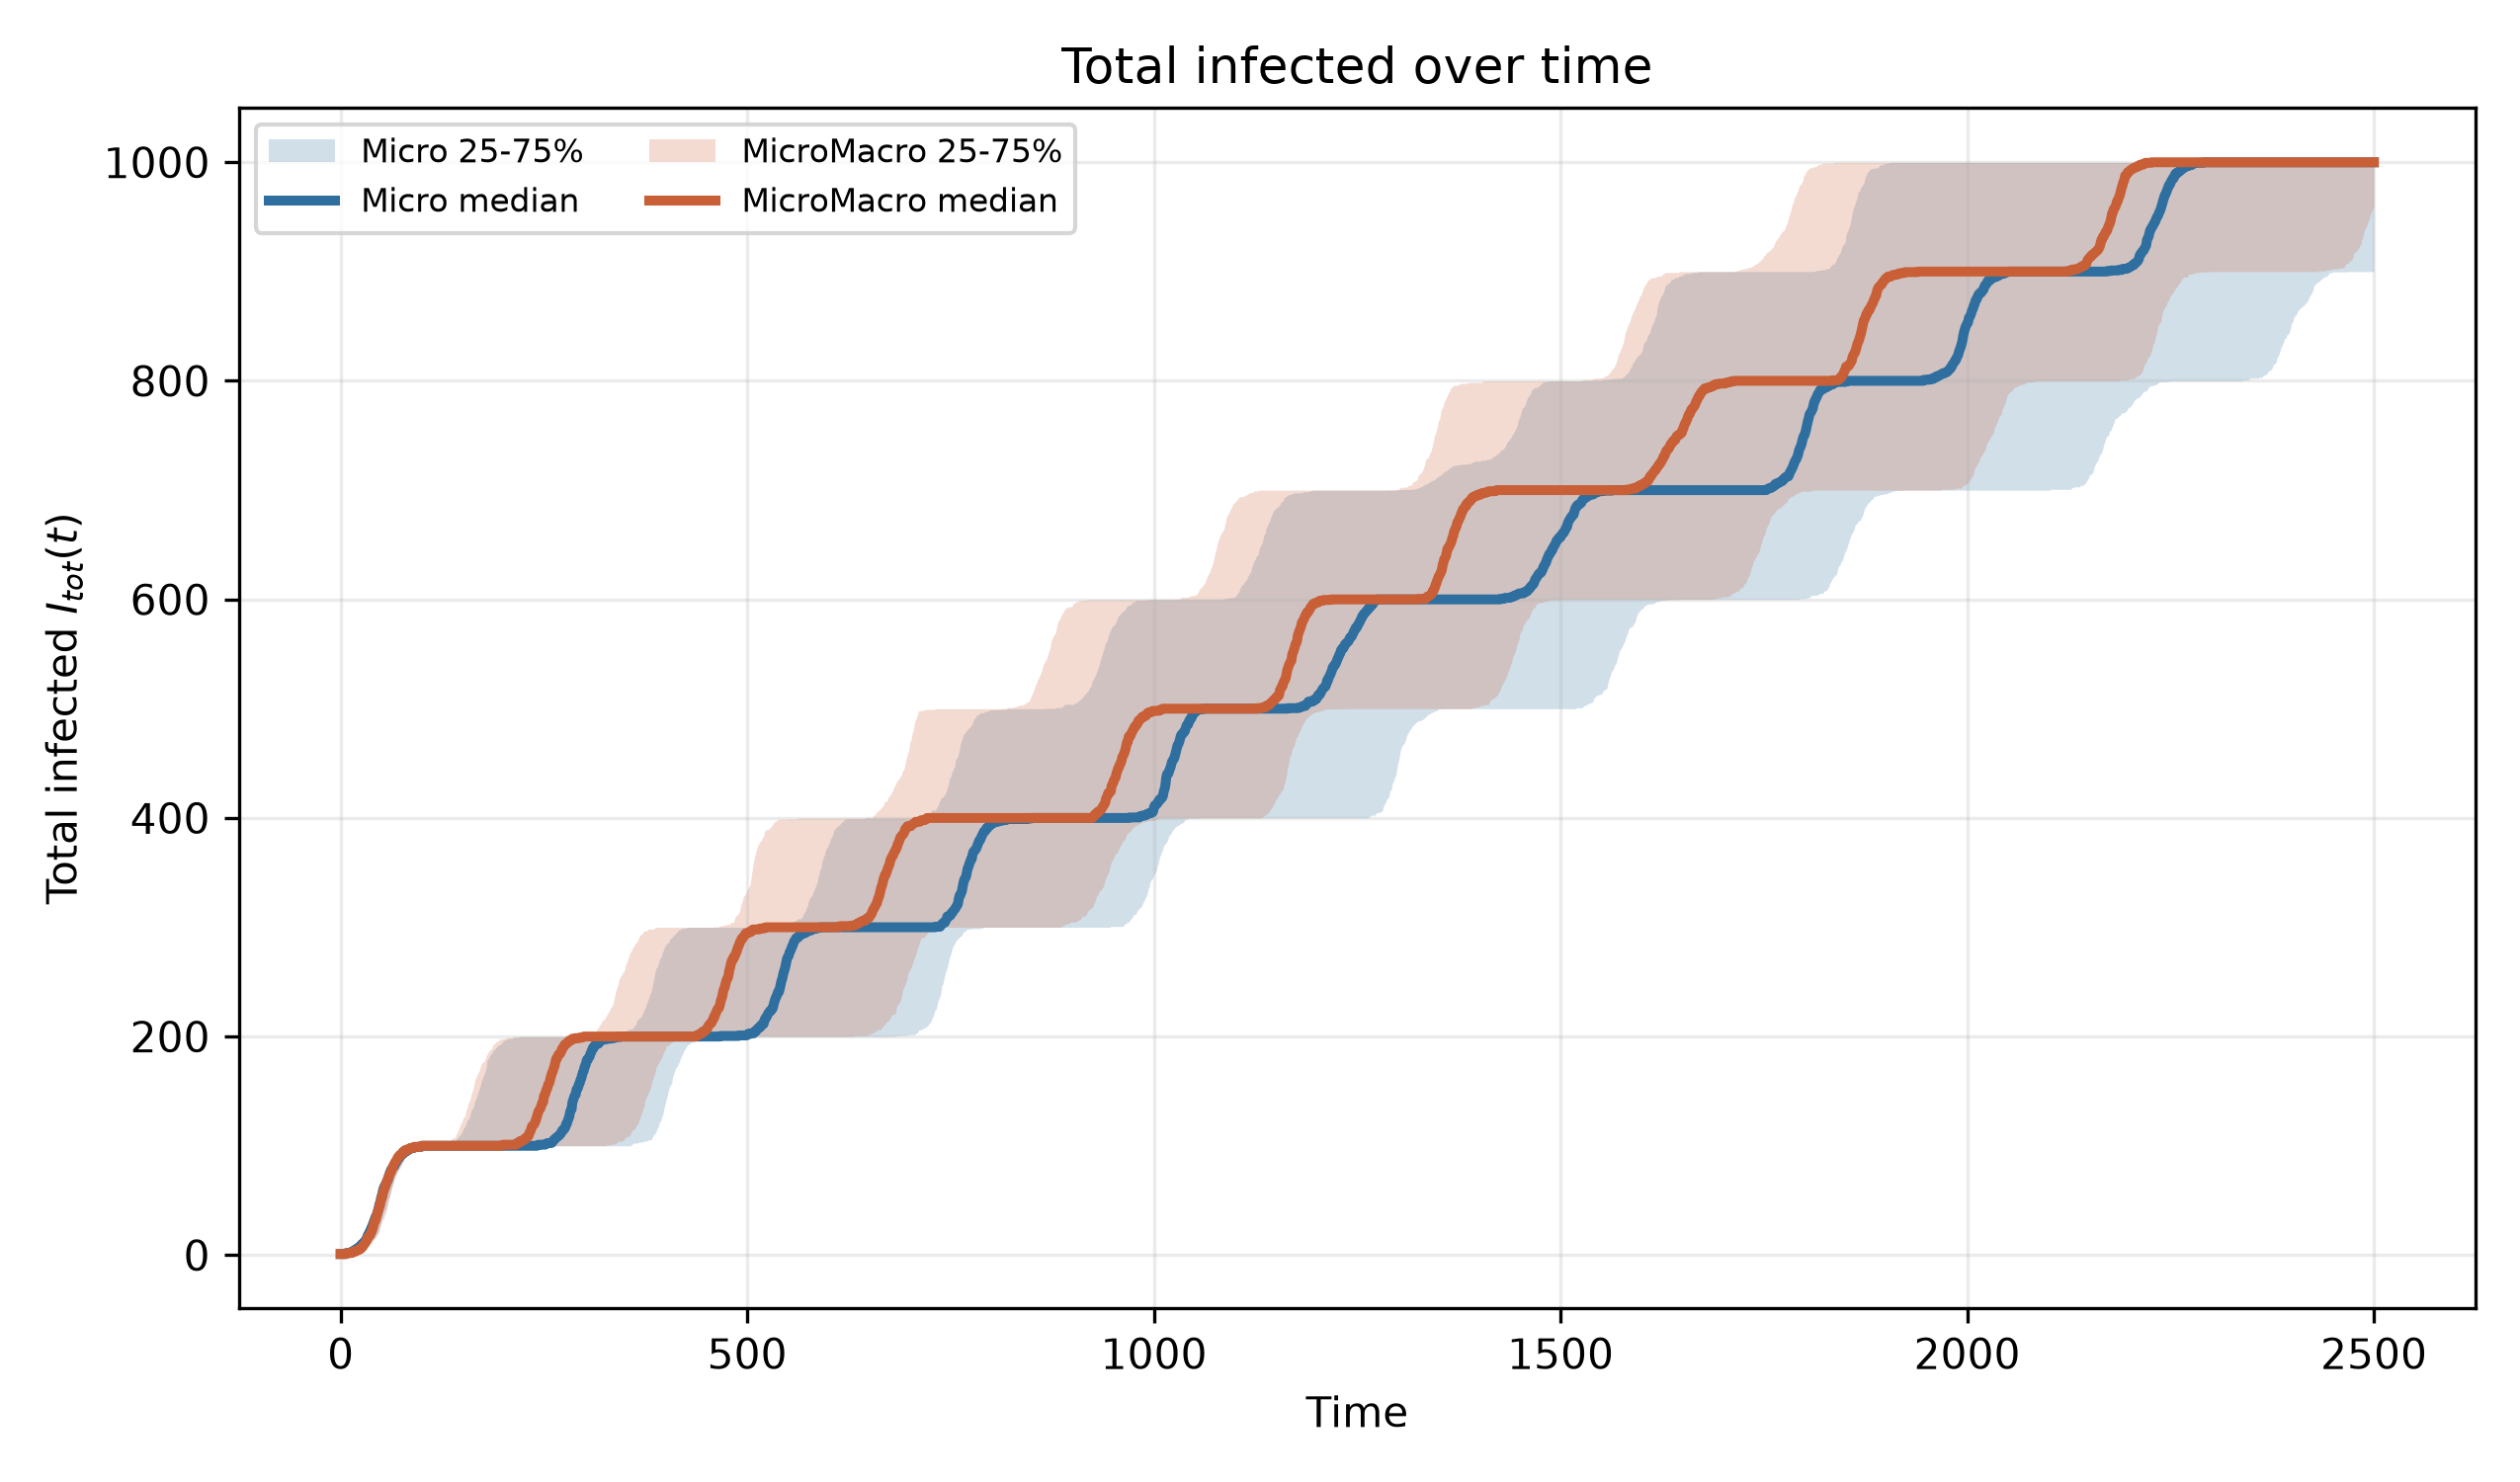
\includegraphics[width=\linewidth]{../../paper/Images/research_synthesis/clique_total_infected_iqr.png}
  \caption{Calibrated clique baseline.}
 \end{subfigure}\hfill
 \begin{subfigure}[t]{.48\linewidth}
  \centering
  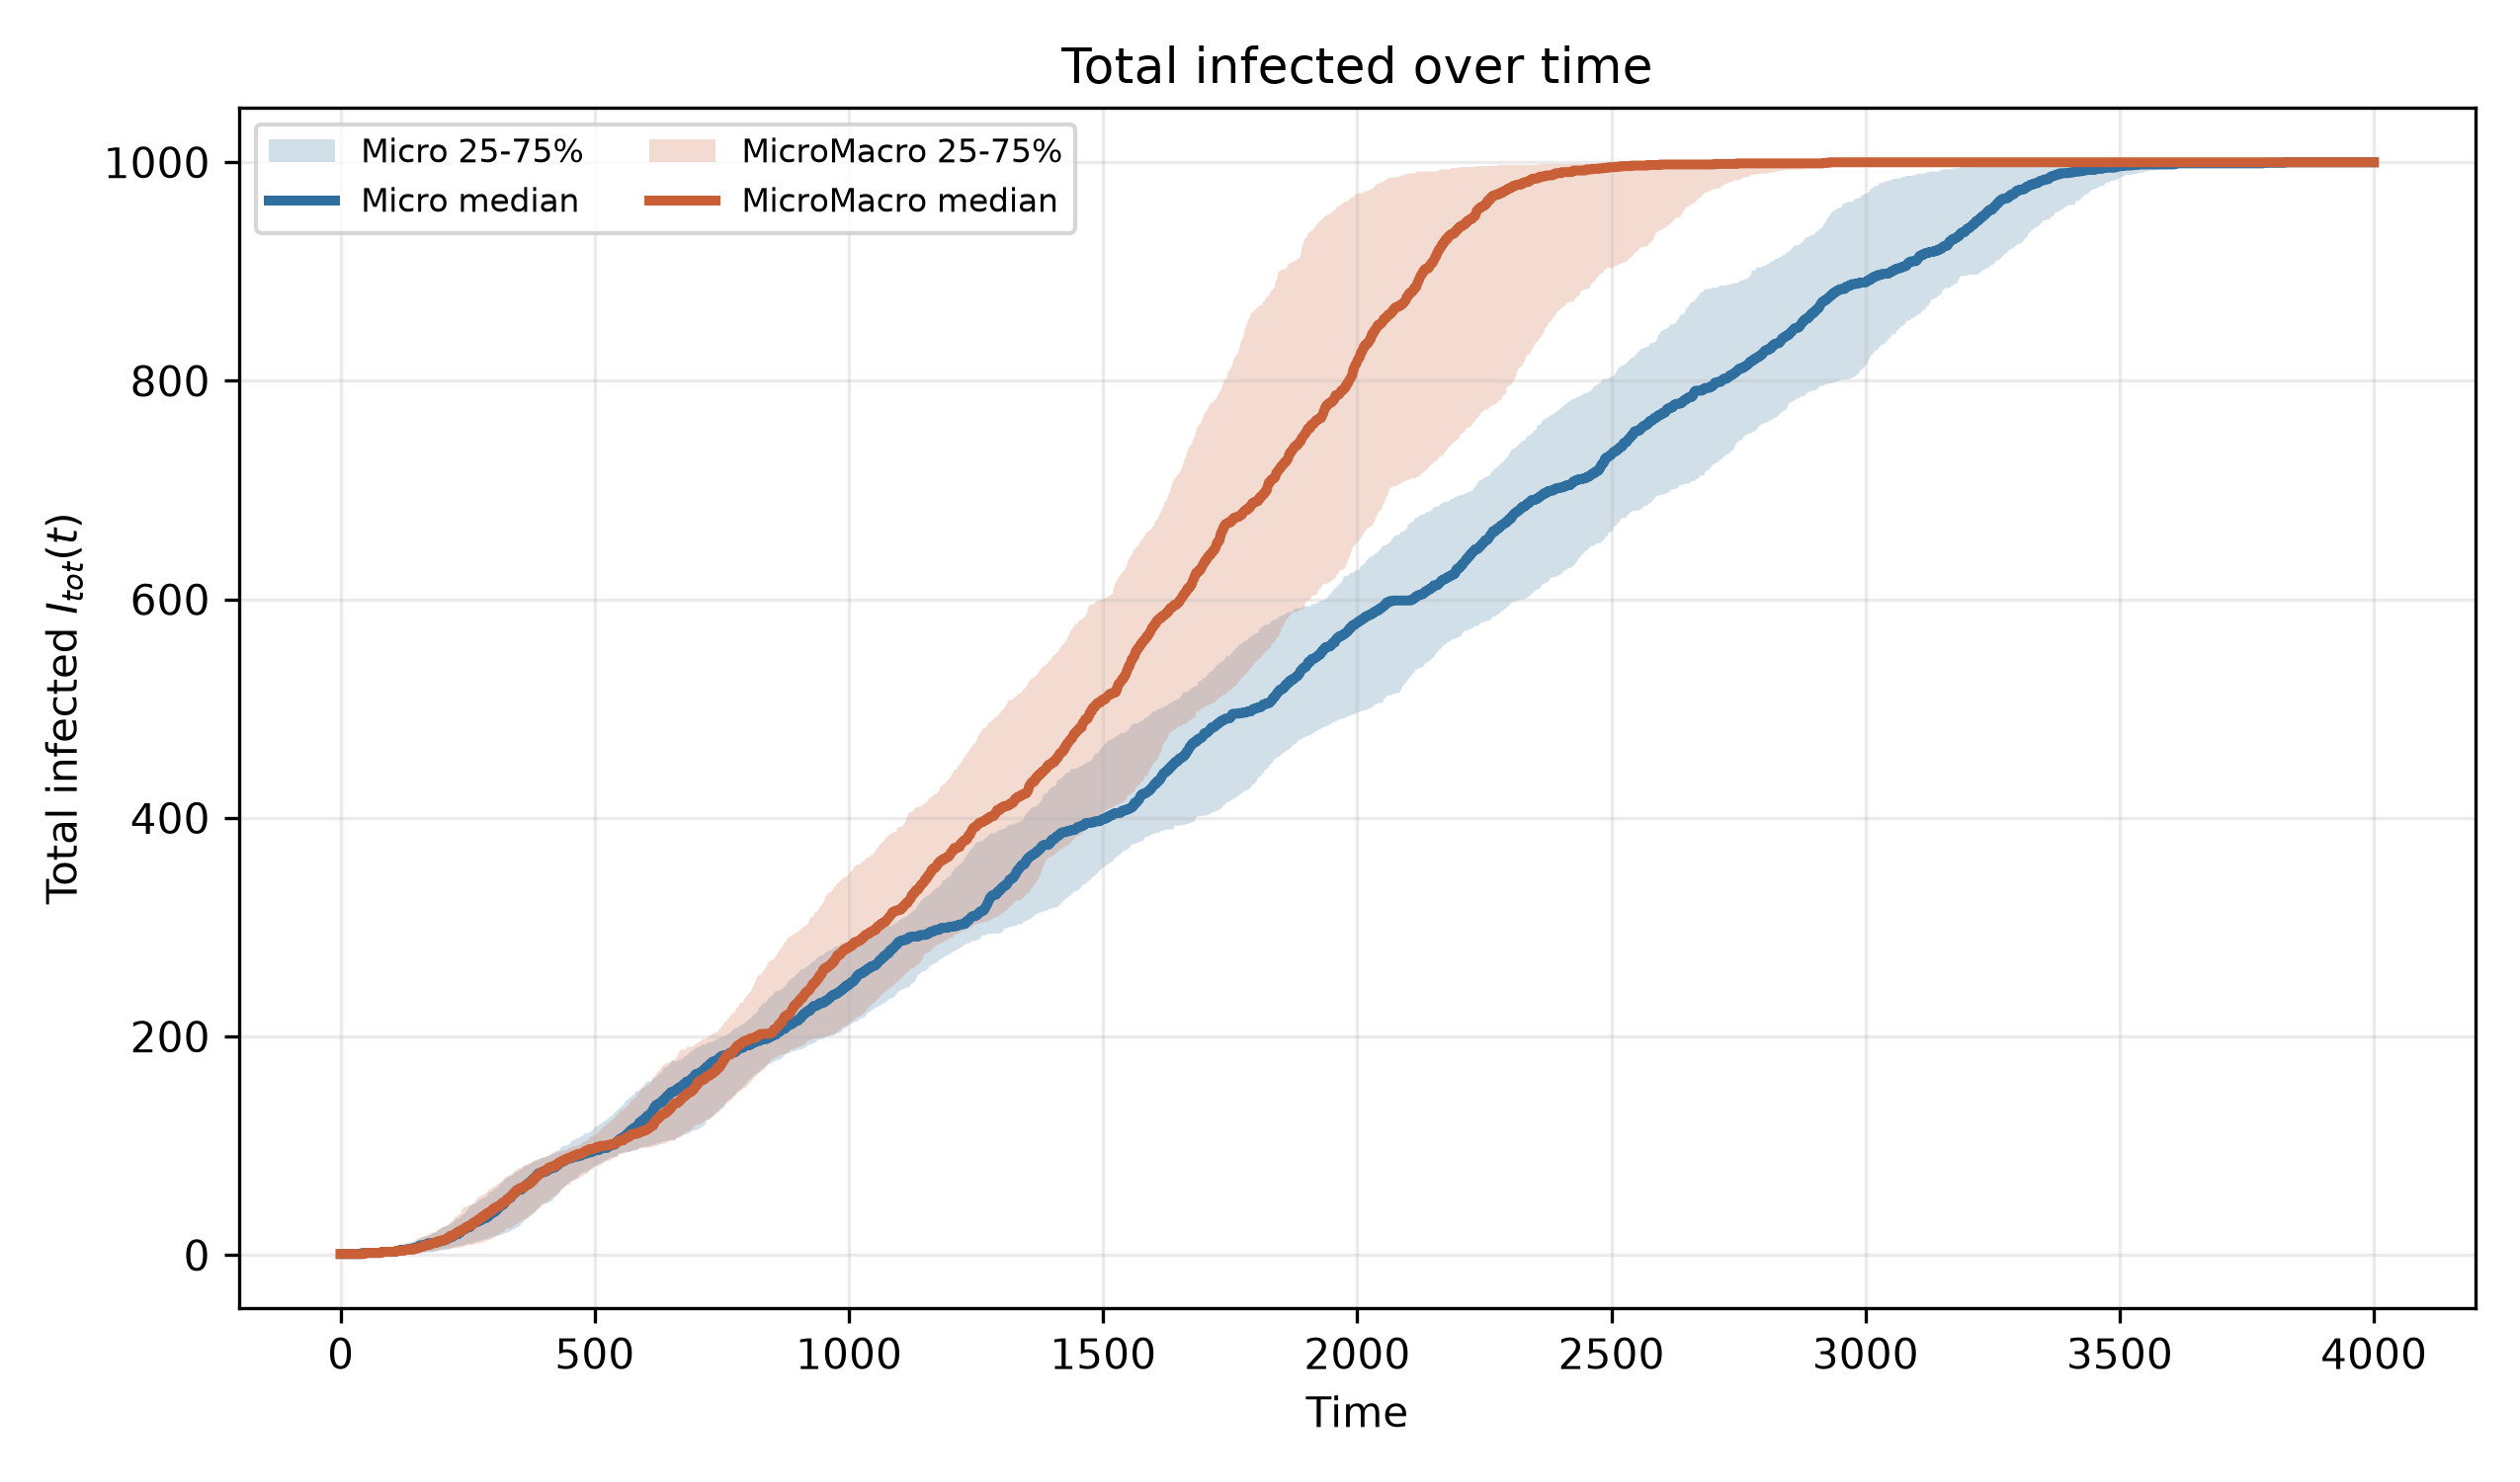
\includegraphics[width=\linewidth]{../../paper/Images/research_synthesis/sparse_total_infected_iqr.png}
  \caption{Sparse connected baseline.}
 \end{subfigure}
 \caption{Aggregate infected trajectories з основної статті. Solid curves ---
 pointwise medians, shaded regions --- interquartile ranges за 100 replications.
 Різні часові шкали й параметри збережені як у відповідних benchmarks.}
\end{figure}

\subsection{Наслідки для калібрування}

Clique і sparse benchmarks не є чистою topology ablation: вони використовують
різні $\beta$ та horizons, тому їхні абсолютні RMST shifts не слід напряму
віднімати. Разом вони задають корисні acceptance regimes. Correction має
залишатися близькою до identity у calibrated clique baseline, але суттєво
зменшувати premature timing і completion mismatch у sparse connected cells.
Немонотонна залежність від $k$ додатково показує, що одного interface width
недостатньо: calibration має враховувати export-to-mixing ratio та внутрішню
reachability.

\section{Що саме створює розбіжність}

\subsection{Rate abstraction: прямо підтверджене джерело premature leakage}

State-replay audit обчислював exact active-edge hazard і aggregate hazard на
одних і тих самих Full Micro states. Середній cumulative exact hazard становив
$27.131$, aggregate --- $46.078$. Mean signed discrepancy mass була $18.947$,
absolute mass --- $25.154$. Over-hazard mass ($22.05$) переважала under-hazard
mass ($3.10$), хоча знак локальної похибки не був постійним.

Найбільш прямий доказ premature leakage: у середньому $22.54\%$ aggregate
cumulative hazard накопичувалося тоді, коли exact active-edge hazard дорівнював
нулю (95\% bootstrap interval $21.56$--$23.61\%$). У ранній фазі відповідна
частка сягала приблизно $79.2\%$. Отже, $I_i/N_i>0$ не означає, що інфекція вже
досягла вузлів, здатних експортувати її до наступної спільноти.

\begin{figure}[H]
 \centering
 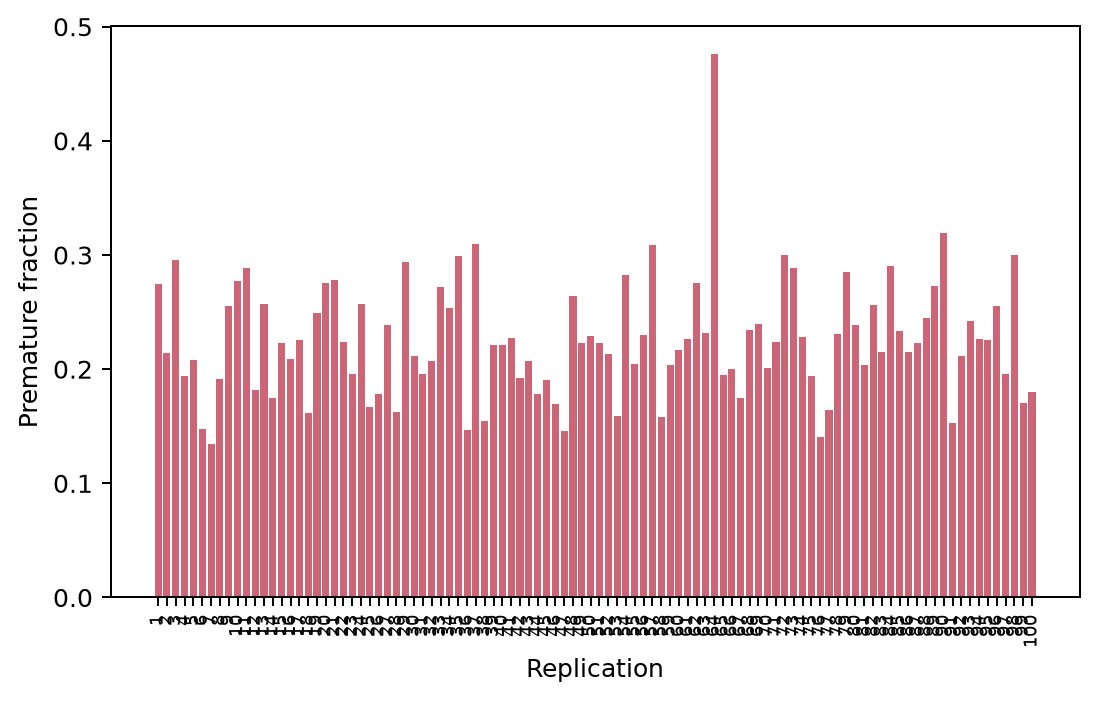
\includegraphics[width=.72\linewidth]{../../paper/Images/research_synthesis/hazard_premature_fraction.png}
 \caption{Частка aggregate cumulative hazard, накопичена за нульового exact
 active-edge hazard. Статистична одиниця --- replication.}
\end{figure}

\subsection{Import placement: важливий, але залежний від hazard context}

Exp-01 показав, що oracle exact-hazard/exact-placement architecture узгоджується
з Full Micro: completion $1.0$, relative $W_1=0.0138$, а
$\Delta\mathrm{RMST}=7.5$ з CI $[-93.6,120.3]$. Це validation gate для
експериментального scheduler.

За exact hazard заміна exact placement на uniform змістила RMST на $-168.8$
($[-274.5,-56.1]$). Aggregate hazard із boundary-aware placement відрізнявся
від exact/exact на $-208.8$ ($[-310.0,-112.2]$). Повна aggregate/uniform
похибка становила $-220.8$ ($[-315.5,-126.8]$). Однак додатковий uniform effect
після aggregate/boundary був лише $-19.6$ і мав CI, що включав нуль.

Ці компоненти не можна додавати: hazard змінює trajectory і множину станів, у
яких placement взагалі відбувається. Крім того, aggregate-hazard/exact-placement
не завжди математично визначений, коли $\lambda_{ij}>0$, але активних exact
edges немає.

\begin{figure}[H]
 \centering
 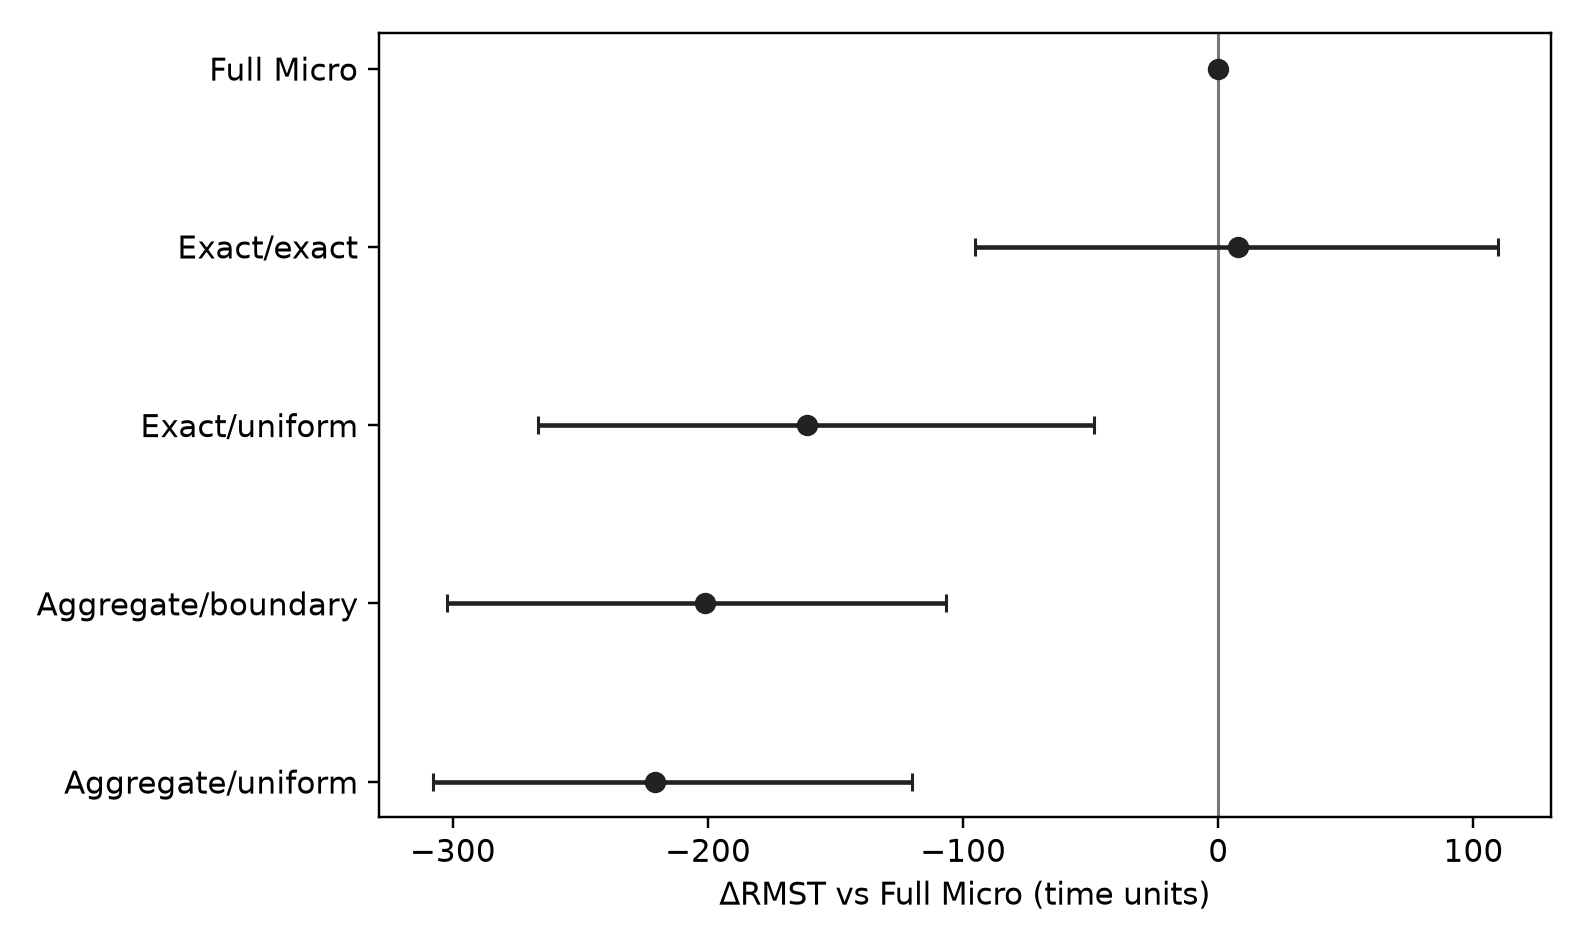
\includegraphics[width=.75\linewidth]{../../paper/Images/research_synthesis/ablation_rmst_shift.png}
 \caption{RMST shifts у hazard--placement ablation. Boundary placement є
 static edge-weighted approximation, а не exact placement.}
\end{figure}

\subsection{Synchronization залишається окремою невизначеністю}

Event-driven aggregate/uniform Exp-01 мав relative $W_1$ близько $7.5\%$,
тоді як production sparse benchmark --- близько $42.6\%$. Відмінність не можна
автоматично приписати synchronization, бо experiments використовували різні
schedulers і endogenous paths. Production-vs-event-driven audit ще не проведено.
Тому midpoint hazard integration і residual-budget semantics залишаються
незакритим джерелом похибки, яке слід відокремити до фінальної калібрації.

\section{Коли похибка мала або змінює знак}

\subsection{Швидке внутрішнє mixing і короткі well-mixed chains}

У dense negative control з трьох cliques, $n=100$, $k=2$ і 200 replications
обидва методи мали completion $1.0$. $\Delta\mathrm{RMST}=8.2$ з CI
$[-39.0,54.4]$, а KS $p=0.545$. Це не формальний equivalence test, але
свідчить проти великого універсального scheduler offset.

\begin{figure}[H]
 \centering
 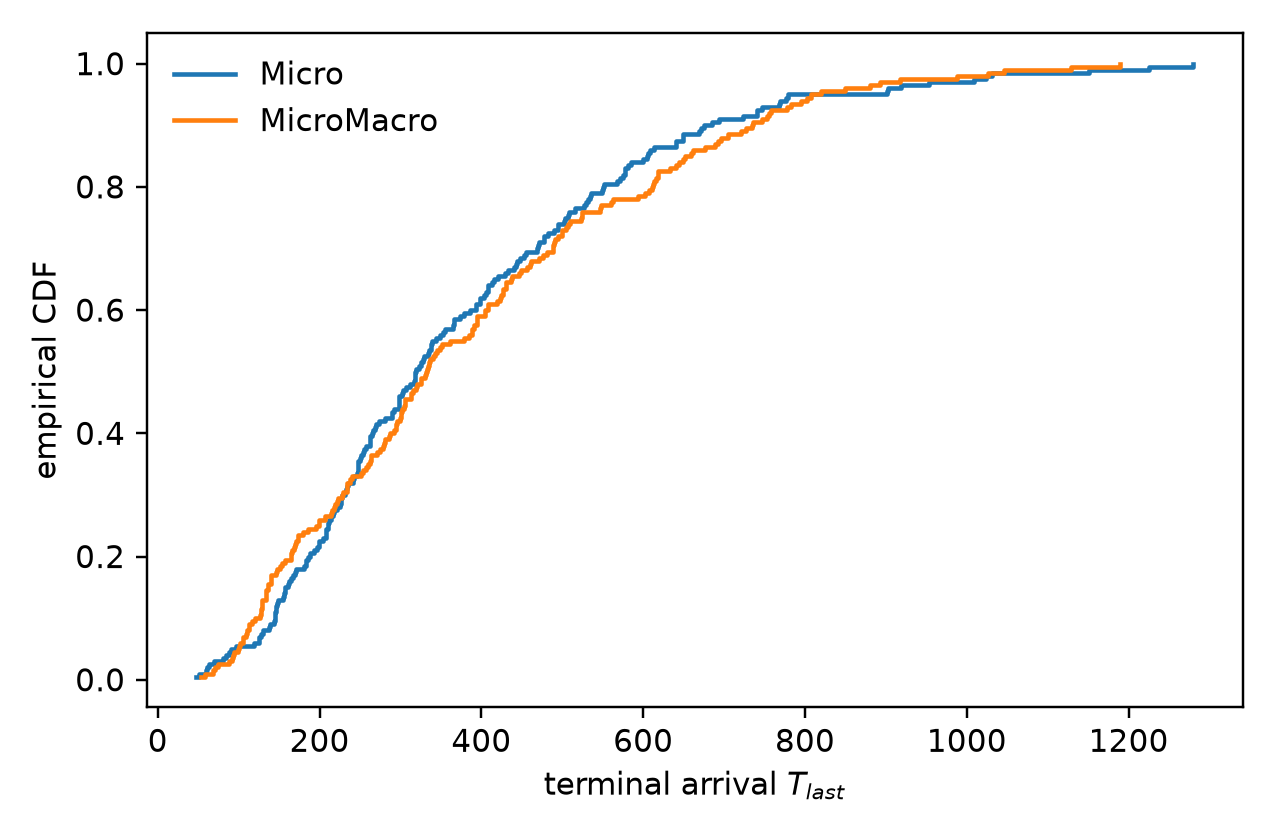
\includegraphics[width=.68\linewidth]{../../paper/Images/research_synthesis/dense_control_terminal_cdf.png}
 \caption{Terminal-arrival distributions у dense negative control.}
\end{figure}

У calibrated chain-of-cliques baseline difference була невеликою відносно
часового масштабу, хоча completion і censoring вимагали обережності. Complete
communities швидко роблять infected fraction репрезентативним для boundary
exposure, тому macro aggregation працює краще.

\subsection{Повільний export усуває premature bias, але не гарантує agreement}

CE-03/CE-11 показав sign change зі зростанням
$r=\beta_{out}/\beta_{in}$. На horizon-aware шкалі normalized RMST shift був
$+0.240$ при $r=0.1$, $+0.056$ при $r=0.3$, $-0.339$ при $r=1$,
$-0.546$ при $r=2$ і $-0.606$ при $r=5$. Отже, slow export дає infection
час перемішатися й досягти gateway nodes до наступної macro події, тому
premature bias зникає. Проте при $r=0.1$ виникає великий late bias, а не
equivalence. У цьому режимі damping не потрібен і може зробити модель ще
повільнішою; correction має вміти змінювати знак або вимикатися.

\section{Коли розбіжність стає великою}

\subsection{Великий export-to-mixing ratio}

CE-06 full охоплював 36 cells із $r\in\{0.5,1,2\}$,
$d\in\{4,6,10,20\}$, $k\in\{2,5,10\}$ і 60 replications у cell. Середній
$\Delta\mathrm{RMST}/T_{end}$ дорівнював $-0.0028$, $-0.1275$ і $-0.3034$
для $r=0.5,1,2$ відповідно. Mean relative $W_1$ зростав від $0.241$ до
$0.543$. Таким чином, $r$ є головним regime descriptor у дослідженій grid.
Майже нульова mean signed error при $r=0.5$ не означає agreement: вона
поєднує cells різного знака, тоді як mean relative $W_1=0.241$ залишається
помітною.

\subsection{Sparse communities і вузькі interfaces}

Після усереднення за іншими параметрами normalized error змінювалася від
$-0.222$ при $d=4$ до $-0.075$ при $d=20$, а зі збільшенням $k$ від 2 до 10
--- від $-0.176$ до $-0.115$. Найгірша cell $(r,d,k)=(2,4,2)$ мала
$-0.528$. Sparse structure збільшує час досягнення конкретних boundary nodes;
вузький interface робить availability ще менш репрезентативною для $I/N$.

\begin{figure}[H]
 \centering
 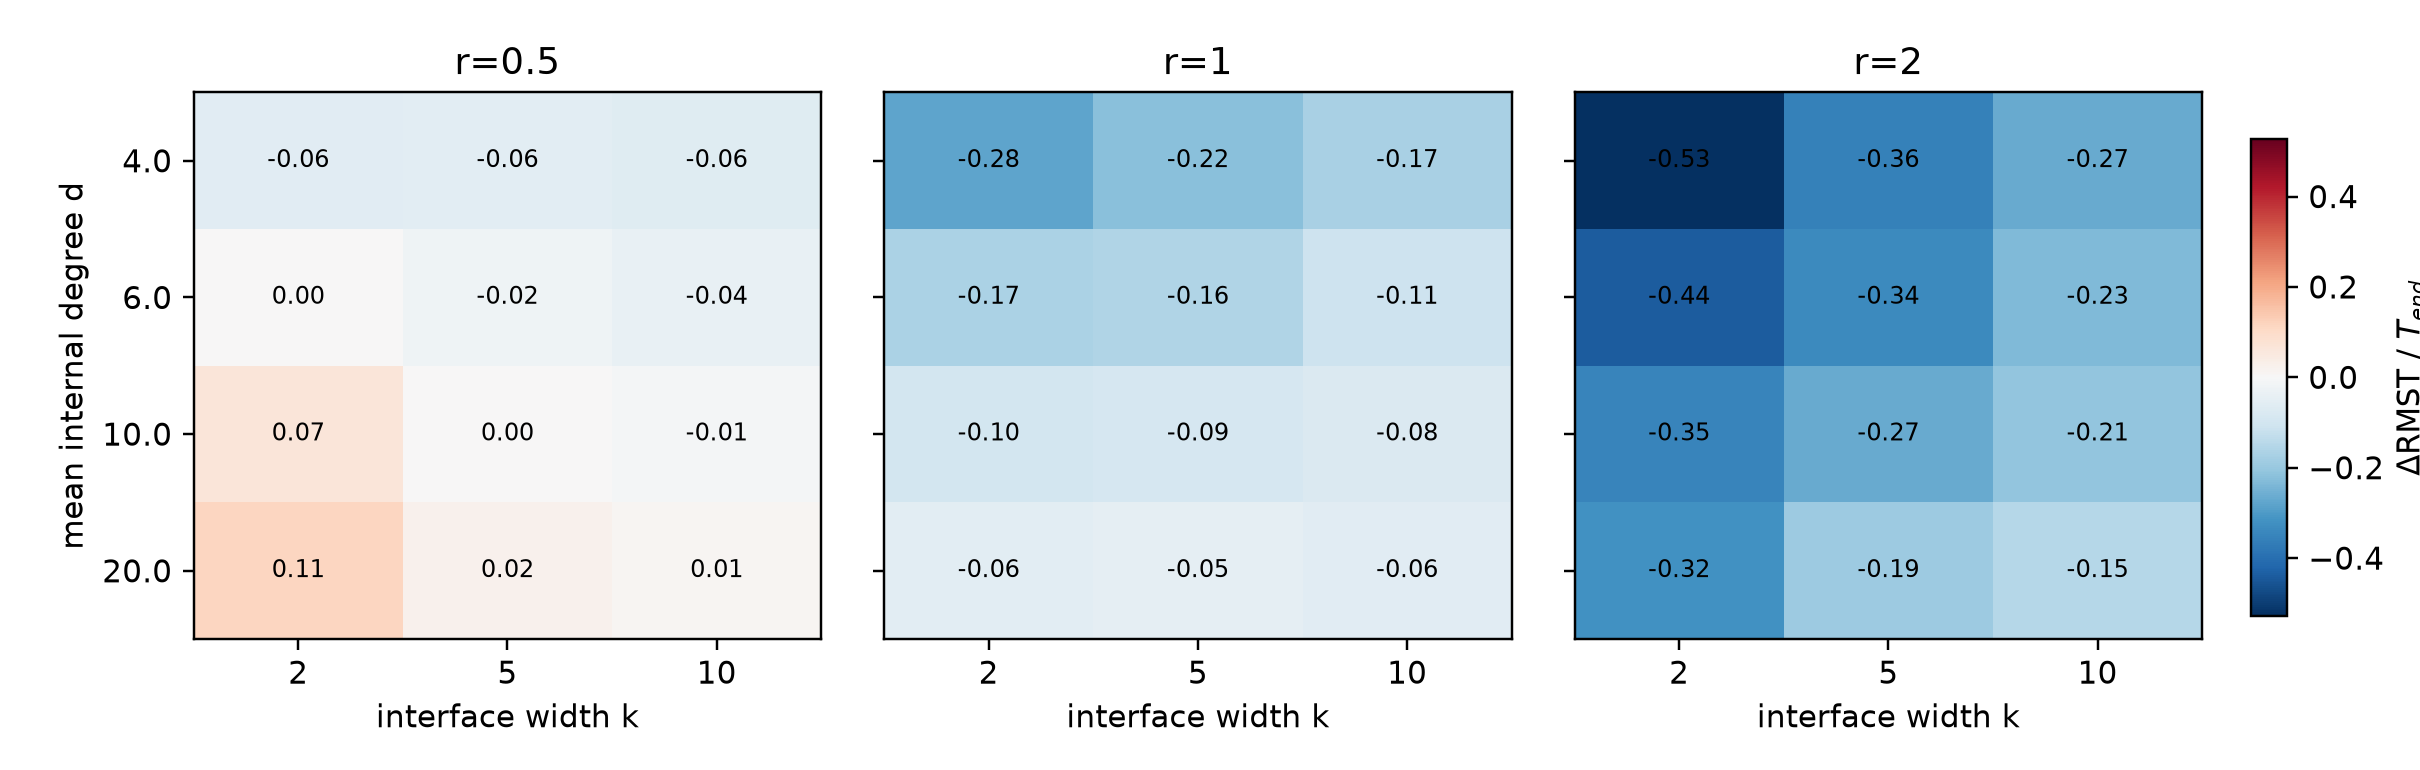
\includegraphics[width=.98\linewidth]{../../paper/Images/research_synthesis/regime_map.png}
 \caption{Regime map normalized RMST error. Від'ємні значення означають
 premature MicroMacro arrivals.}
\end{figure}

\subsection{Довгі chains накопичують локальну похибку}

Layer-wise comparisons показують, що discrepancy зростає вздовж sparse chain.
Навіть помірний local-delay shift повторюється на кількох interfaces і стає
великим terminal-arrival error. Тому калібрування лише за $T_{last}$ може
приховати, на якому layer починається систематичне відхилення; потрібні також
$T_i$ і $\Delta T_i$.

\subsection{Recovery змінює не лише timing, а й outbreak probability}

CE-04 порівняв SI та SIR. $\Delta\mathrm{RMST}$ змінився від $-1068$ при
$\gamma=0$ до $-1726$ при $\gamma=0.003$. При $R_0=1$ Full Micro завершив
chain propagation у $28\%$ runs, MicroMacro --- у $72\%$, тобто completion gap
становив 44 percentage points. У recovery regimes completed-only arrival
distribution вже не описує головну помилку: модель може передбачити downstream
outbreak там, де stochastic reference згасає.

\section{Що показали спроби корекції}

\subsection{Scalar calibration: корисний перший рівень, але не розв'язання}

CE-07 pilot підбирав multiplier $c$ для $\beta_{macro}$ у дев'яти $(r,d)$
cells. Absolute normalized error покращився у всіх cells, але $c^*$ змінювався
від $0.5$ до $1.2$. Mean residual structural fraction була приблизно $0.43$ при
$r=0.5$, $0.37$ при $r=1$ і $0.71$ при $r=2$.

Оскільки $c^*$ вибирався й оцінювався на тих самих 40 replications, це
оптимістична development estimate. Висновок: scalar calibration має бути
baseline layer, але не може замінити state-dependent correction.

\subsection{Spectral damping: правильний напрям лише в частині regimes}

CE-10 застосовував $\alpha=\mathrm{clamp}(1/\mu_2,1,6)$ у
$(I/N)^\alpha$. При $r=2$ mean gap closure становила $0.675$, а найкраща cell
досягла $0.933$. При $r=1$ mean closure була $0.403$. Проте при $r=0.5$
correction перетворила майже нульову mean error $-0.0128$ на late error
$+0.1262$; mean gap closure стала $-3.38$. Загалом покращилися 7 із 12 cells.

\begin{figure}[H]
 \centering
 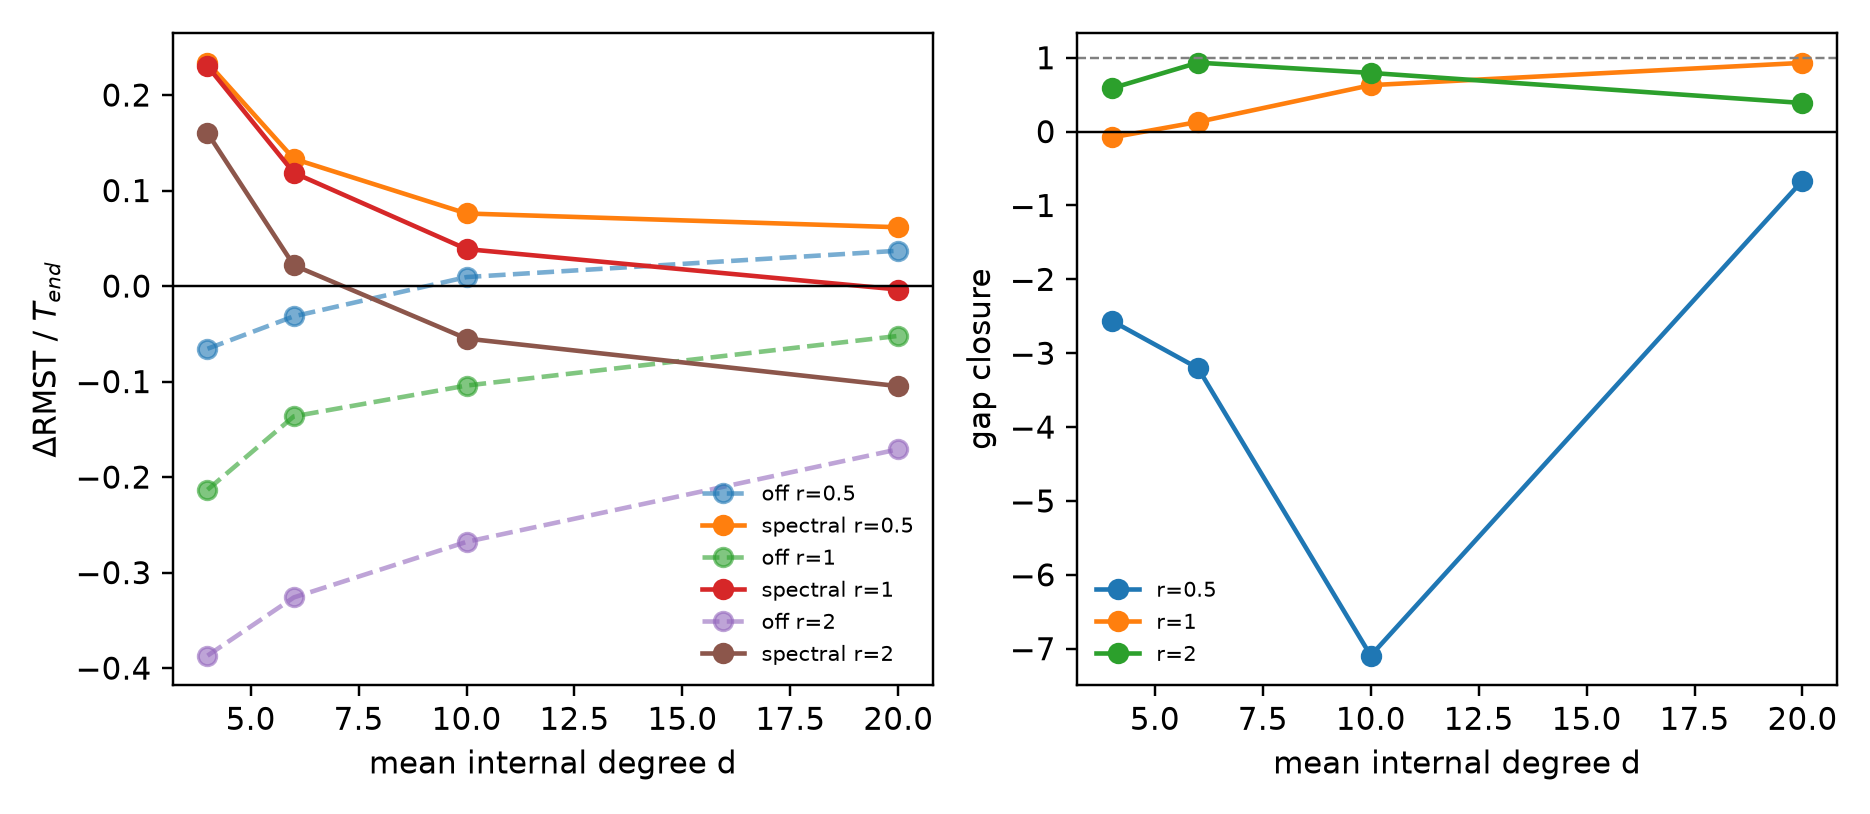
\includegraphics[width=.9\linewidth]{../../paper/Images/research_synthesis/spectral_correction.png}
 \caption{Spectral correction допомагає у fast-export regime і регресує у
 slow-export regime.}
\end{figure}

Це прямий доказ, що spectral descriptor має керувати силою correction разом
із $r$, але не може бути always-on exponent.

\subsection{Static boundary placement не є універсальною заміною}

CE-09 boundary placement зменшив absolute normalized RMST лише в одній із
шести $(d,k)$ cells; у dense cells correction могла змінити premature bias на
late bias. Boundary membership саме по собі не описує distance від поточного
infected set, internal degree gateway і доступність наступного interface.

Цей експеримент не є чистою causal placement ablation: modes використовували
різні network seed blocks, а oracle exact одночасно змінював hazard і placement.
Тому numerical contrasts між modes є diagnostics, а не paired causal effects.

\subsection{Literal lag і latent-boundary corrections були надто сильними}

Experiment 05 validation перевіряв fixed spectral lag, latent relaxation та
їх комбінацію. Baseline production variant завершив усі runs із relative
$W_1=0.091$. Lag і combined variants не мали terminal completions, а latent
variant завершив $55\%$ і мав relative completed-only $W_1=0.200$. Жодна
literal correction не покращила validation result. Final robustness sweeps
залишаються незавершеними й не використовуються у цьому синтезі.

Наслідок не в тому, що delay mechanism неправильний, а в тому, що fixed
spectral formula без calibration та regime gate надмірно гальмує export.

\subsection{Multi-topology validation є обов'язковим acceptance gate}

ER-01 smoke показав, що parameters-only C2/C12 можуть працювати на
random-connected і complete cases, але регресувати на clique-leaves. Pilot
на 54 cells зараз виконується, тому partial outputs не використовуються для
фінальних claims. Correction, що покращує середній sparse-chain baseline, але
погіршує іншу topology family, не може вважатися готовою.

\section{Комплексна інтерпретація всього evidence chain}

\subsection{Де результати взаємно підсилюють один одного}

Сукупний доказ складається з послідовних рівнів. B00 показує, чому втрата
bridge identity здатна змінити survival distribution навіть за коректного
conditional mean hazard. B01 демонструє, що цей механізм може бути слабким у
fast-mixing clique regime. B02 показує великий production-level effect після
введення sparse internal reachability. Exp-02 далі підтверджує formula mismatch
на спільних microscopic states, а Exp-01 показує, що і hazard abstraction, і
placement можуть причинно змінювати arrival timing. CE-03/11 та CE-06 встановлюють,
що величина і знак outcome error залежать від export-to-mixing regime. CE-04
показує, що recovery переносить проблему з timing на probability of propagation.
Нарешті, CE-07, CE-09, CE-10 та Exp-05 демонструють, чому одна scalar,
boundary-only або always-on spectral correction не є достатньою.

Цей ланцюг підтримує висновок про boundary information loss на трьох різних
рівнях: analytical event clock, common-state hazard replay і endogenous
full-system trajectories. Жоден окремий experiment не дає всього висновку;
сила аргументу походить саме з їх узгодження.

\subsection{Де результати не можна звести до простої історії}

\paragraph{Early-bias theorem проти late regimes.}
Jensen argument у B00 передбачає premature mean-field export за своїх
exchangeability та conditional-mean assumptions. CE-03/11, однак, дає
$\Delta\mathrm{RMST}>0$ при $r=0.1$ і $0.3$. Це не спростовує theorem:
production simulator має endogenous imported states, synchronization,
placement і calibrated rates, а conditioning після survival selection вже не
збігається з мінімальною постановкою. Практичний висновок --- correction не
може бути завжди damping-only; спершу потрібен sign/regime gate.

\paragraph{Interface width не є одновимірним predictor.}
Вузький $k$ збільшує boundary localization і censoring, але більший $k$ також
прискорює repeated export та може збільшити відносну discrepancy. У clique
sweep relative $W_1$ зросла від $0.035$ при $k=5$ до $0.160$ при $k=20$; у
sparse sweep значення залишались великими при $k=10,20$. CE-06 в середньому
показує покращення зі зростанням $k$, але не універсальну монотонність.
Отже, $k$ слід використовувати лише разом із $r$, $d$, $N$ і mixing proxy.

\paragraph{Placement effect залежить від hazard path.}
За exact hazard uniform placement дав значущий shift $-168.8$, але після
aggregate hazard додатковий uniform effect був лише $-19.6$ з CI, що включав
нуль. CE-09 також не підтвердив static boundary placement як універсальне
покращення. Це означає, що ``boundary error'' не можна зводити тільки до target
node: головною прихованою змінною є joint process event timing, source state і
post-import microstate.

\paragraph{Event-driven і production magnitudes не узгоджені.}
Event-driven aggregate/uniform Exp-01 мав relative $W_1\simeq0.075$, тоді як
production B02 baseline мав $0.426$. Вони використовують споріднений sparse
regime, але різні scheduler semantics. До paired production-vs-event-driven
audit не можна визначити, чи різниця походить від midpoint quadrature,
event-time marking, residual budget, trajectory coupling або їх interaction.
Це найбільша незакрита attribution gap.

\subsection{Що відомо про corrections у сукупності}

\begin{table}[H]
\centering
\caption{Статус перевірених correction families. ``Benefit'' не означає
generalization поза перевіреним дизайном.}
\begin{tabular}{p{3.2cm}p{4.0cm}p{4.0cm}p{3.2cm}}
\toprule
Correction & Де допомагає & Де не працює & Статус\\
\midrule
Scalar $c\beta_{macro}$ & усі 9 CE-07 pilot cells in-sample & $c^*=0.5$--$1.2$; structural residual & development\\
Spectral exponent C1 & $r=1,2$ random-connected; 7/12 cells & strong late regression при $r=.5$ & regime-specific\\
Static boundary placement & окремі sparse cells & 5/6 CE-09 regimes без покращення; unpaired design & diagnostic\\
Boundary/renorm C2/C12 & ER-01 smoke random-connected/complete & regression на clique-leaves & generalization failed at smoke\\
Fixed lag/latent Exp-05 & жодного baseline improvement & zero/low terminal completion & rejected literally\\
\bottomrule
\end{tabular}
\end{table}

Спільний висновок correction experiments є негативним, але корисним: error не
контролюється одним static descriptor або одним global multiplier. Перспективна
модель повинна оцінювати regime, плавно вимикатися в identity/late cells і
використовувати state-dependent availability лише там, де export випереджає
mixing. Це ще design requirement, а не підтверджений алгоритм.

\subsection{Рівень доказовості основних тверджень}

\small
\setlength{\tabcolsep}{4pt}
\begin{longtable}{p{5.5cm}p{2.0cm}p{5.5cm}}
\toprule
Твердження & Рівень & Головне обмеження\\
\midrule
MicroMacro може давати practically large premature arrival у sparse chains & високий & Доведено для SI random-connected family.\\
Boundary-dependent aggregate hazard є реальним механізмом & високий & Outcome contribution поза baseline залежить від scheduler/regime.\\
Rate abstraction важливіша за placement & середньо-високий & Один causal baseline; effects неадитивні.\\
$r$ та mixing визначають знак і magnitude error & високий у grid & Threshold не валідований на інших topology families.\\
Recovery збільшує completion mismatch & середній & Одна network family і обмежена $\gamma$ grid.\\
Поточні C1/C2/C12 є deployable corrections & відхилено & Немає minimax multi-topology validation.\\
Production scheduler пояснює розрив $0.075$ vs $0.426$ & невідомо & Прямий synchronization audit відсутній.\\
\bottomrule
\end{longtable}
\normalsize

\section{Синтез: предиктори розбіжності}

\begin{table}[H]
\centering
\caption{Практичні regime descriptors для майбутнього calibration model.}
\begin{tabular}{p{3.1cm}p{4.2cm}p{7.0cm}}
\toprule
Descriptor & Очікуваний напрям & Evidence\\
\midrule
$r=\beta_{out}/\beta_{in}$ & $r\uparrow$: більше premature bias & CE-03, CE-06, CE-11, CE-10\\
Mixing proxy $\mu_2$ & $\mu_2\uparrow$: менша потреба у damping & CE-06, CE-08, CE-10\\
Mean degree $d$ & $d\uparrow$: менший boundary-reach delay & Sparse benchmark, CE-06\\
Interface width $k$ або $k/N$ & effect немонотонний; визначає localization і export clock & Chain sweeps, CE-06\\
Boundary fraction & мала частка: потенційно більша mismatch & Exp-01, CE-09; сама по собі недостатня\\
Boundary internal degree & high degree може прискорити reachability & ER-01 smoke failure analysis\\
Recovery ratio $\gamma/\beta$ & recovery підсилює completion mismatch & CE-04\\
Chain position $i$ & error накопичується downstream & Chain benchmarks, Exp-01 layer metrics\\
\bottomrule
\end{tabular}
\end{table}

Найкорисніший узагальнений descriptor має порівнювати export clock із mixing
clock, а не використовувати їх окремо. Концептуально це quantity виду
\[
 z_i = \frac{\beta_{out}\,w_i}{\beta_{in}\,m_i},
\]
де $w_i$ --- нормована interface exposure, а $m_i$ --- parameters-only mixing
proxy на основі $\mu_2$, degree moments або calibrated reach time. Точна форма
ще не ідентифікована; наведений вираз є design principle, не встановленою
формулою.

\section{Рекомендована архітектура калібрування}

\subsection{Рівень 1: regime classification і identity gate}

Перед застосуванням correction визначати режим за
$r$, $\mu_2$, $d$, $k/N$, boundary fraction і, для SIR, $\gamma/\beta$.
У slow-export або well-mixed regime correction повинна плавно переходити в
identity. Negative-control критерій: dense clique-like cells не мають отримувати
practically relevant regression.

\subsection{Рівень 2: scalar calibration}

Підібрати $c(\mathbf{x})$ у
\[
 \lambda^{cal}_{ij}=c(\mathbf{x}_i)\lambda^{ref}_{ij},
\]
де $\mathbf{x}_i$ містить лише дозволені aggregate descriptors. Це усуває
систематичну rate-scale component, але не state-dependent boundary lag.
Training і evaluation seed blocks повинні бути розділені; CE-07 in-sample
$c^*$ не можна використовувати як unbiased performance estimate.

\subsection{Рівень 3: gated state-dependent correction}

У fast-export/sparse regime потрібен bounded correction виду
\[
 \lambda^{corr}_{ij}(t)=\lambda^{ref}_{ij}(t)
 \left[1-g(\mathbf{x}_i)\bigl(1-\phi_i(t)\bigr)\right],
\]
де $g\in[0,1]$ --- regime gate, а $\phi_i(t)\in[0,1]$ --- state-dependent
availability proxy. Gate не дозволяє correction діяти в режимах, де baseline
вже accurate або late. Availability proxy не повинна використовувати exact
gateway identities; допустимі spectral/degree/boundary-count statistics.

Це загальна architecture, а не підтверджена конкретна формула. C1, C2 і C12
можуть розглядатися як candidate components після ER-01, але жодна ще не
пройшла minimax acceptance.

\subsection{Рівень 4: окрема calibration для completion у SIR}

За recovery timing correction недостатня. Потрібно одночасно калібрувати
terminal survival/completion probability, оскільки MicroMacro може створювати
false downstream outbreaks. Acceptance objective має містити $\Delta p$ або
survival likelihood, а не лише completed arrival times.

\section{Статистичний protocol для вибору correction}

Рекомендований evaluation protocol:
\begin{enumerate}
 \item paired networks та initialization для Full Micro і всіх variants;
 \item незалежні replication-level bootstrap intervals;
 \item RMST і completion як primary censoring-aware outcomes;
 \item relative $W_1$ лише разом із completion;
 \item train/validation/test split за replication seeds та topology families;
 \item identity penalty на dense negative controls;
 \item minimax criterion за topology/regime, а не найкращий average result;
 \item окремі layer-wise diagnostics для локалізації accumulation;
 \item predeclared equivalence bound, наприклад
 $\epsilon=0.05\,\mathrm{mean}(T_{last}^{Micro})$;
 \item заборона порівняння різних horizons/censoring rules як одного experiment.
\end{enumerate}

Можливий calibration loss на validation set:
\[
 \mathcal{L}=w_R|\Delta\mathrm{RMST}|/T_{end}
 +w_W\mathrm{rel}W_1+w_p|\Delta p|+w_I\mathcal{P}_{identity},
\]
але final selection слід робити за worst-case loss між topology/regime cells.

\section{Що вже можна стверджувати}

\begin{enumerate}
 \item MicroMacro не має одного універсального bias: знак залежить від
 export-to-mixing regime.
 \item Найбільш надійно встановлений механізм premature bias --- aggregate
 hazard до фактичної активності boundary edges.
 \item Import placement важливий, але його ефект залежить від hazard context.
 \item Sparse communities, narrow interfaces, fast export, довгі chains і
 recovery збільшують practically relevant discrepancy.
 \item Well-mixed dense communities є identity regime, де сильна correction
 непотрібна й небезпечна.
 \item Scalar calibration зменшує частину помилки, але structural residual
 залишається і зростає у fast-export regimes.
 \item Spectral information корисна як gate/strength descriptor, але не як
 always-on exponent або fixed lag.
 \item Жодна поточна parameters-only correction ще не пройшла повний
 multi-topology minimax validation.
\end{enumerate}

\section{Що поки не можна стверджувати}

Немає достатніх підстав:
\begin{itemize}
 \item приписувати різницю production benchmark лише synchronization;
 \item називати CE-09 чистою causal placement decomposition;
 \item підтверджувати spectral lag або latent-state hypotheses за Exp-05;
 \item переносити SI calibration на SIR без completion model;
 \item вважати C1/C2/C12 generalizable до завершення ER-01;
 \item робити speedup claims із diagnostic runtimes;
 \item обирати universal calibration constant з CE-07 pilot.
\end{itemize}

\section{Пріоритети наступних кроків}

\begin{enumerate}
 \item Завершити ER-01 pilot і оцінити worst-case gap closure, особливо на
 clique-leaves та slow-export controls.
 \item Завершити CE-07 full із held-out або nested calibration, щоб отримати
 unbiased structural floor.
 \item Провести production-vs-event-driven synchronization audit на тих самих
 networks/seeds/horizons.
 \item Провести gateway-distance experiment, який безпосередньо перевіряє
 reachability mechanism при фіксованих $n,m,d,k$.
 \item Провести replication-power calibration для cells із великим censoring.
 \item Лише після цих gates fitting gated correction і зовнішня topology
 validation можуть вважатися фінальним calibration experiment.
\end{enumerate}

\section{Загальний висновок}

Full Micro і MicroMacro найбільше відрізняються тоді, коли macro export clock
працює швидше, ніж infection встигає перемішатися всередині community і
досягти вузького export interface. Aggregate fraction $I/N$ у такому режимі
є передчасним proxy boundary contagiousness. Якщо mixing швидке або export
повільний, proxy стає репрезентативним і correction повинна вимикатися.

Отже, мета калібрування --- не підібрати один $\beta_{macro}$ для всіх мереж,
а навчитися розпізнавати regime та оцінювати effective boundary availability
за доступними aggregate descriptors. Найбільш захищена стратегія ---
ієрархічна: identity gate, regime-specific scalar calibration, bounded
state-dependent correction і окрема completion calibration для SIR. Її слід
приймати лише за paired censoring-aware та minimax multi-topology validation.

\appendix
\section{Джерела синтезу}

\begin{itemize}
 \item \texttt{paper/main.tex}, calibrated clique та sparse-connected benchmarks
 \item \texttt{reports/ablation\_hazard\_placement/ablation\_report.pdf}
 \item \texttt{reports/experiment\_02\_state\_replay\_hazard\_audit/report.pdf}
 \item \texttt{reports/experiment\_05\_spectral\_corrections/report.pdf}
 \item \texttt{reports/claude\_experiments/ce01\_ablation/}
 \item \texttt{reports/claude\_experiments/ce03\_beta\_ratio/}
 \item \texttt{reports/claude\_experiments/ce04\_sir\_validation/}
 \item \texttt{reports/claude\_experiments/ce06\_regime\_map/}
 \item \texttt{reports/claude\_experiments/ce07\_calibration\_floor/}
 \item \texttt{reports/claude\_experiments/ce08\_negative\_control/}
 \item \texttt{reports/claude\_experiments/ce09\_boundary\_isolation/}
 \item \texttt{reports/claude\_experiments/ce10\_correction\_ladder/}
 \item \texttt{reports/claude\_experiments/metrics\_guide/}
 \item \texttt{docs/ce11\_horizon\_reanalysis/report.md}
 \item \texttt{docs/TODO\_experiments.md} та
 \texttt{docs/experiment\_plan\_error\_reduction.md}
 \item \texttt{docs/error\_reduction\_research/} та
 \texttt{docs/EXPERIMENT\_STATUS.md}
\end{itemize}

\end{document}
